\section{Результаты декомпозиции}
В процессе анализа результатов двумерной декомпозиции был сделан вывод о том, что не для всех галактик "золотой"\textrm{ } выборки полученные модели являются достоверным приближением распределения их поверхностной яркости. Некоторые галактики требуют введения более сложных моделей (учитывающих изломы диска  или же угол наклона относительно луча зрения). Из выборки  галактик, с которыми производилась фотометрическая декомпозиция (73 галактики), 51 галактика имеет адекватно построеную модель, остальные требуют введения более сложных 3D моделей (все дальнейшие шаги производились именно с подвыборкой галактик, имеющих хорошие результаты фотометрической декомпозиции -- 51 галактика). 

Прежде, чем переходить к анализу, мы решили сравнить звездные величины модельных галактик со звездными величинами из базы данных SDSS\footnote{\url{http://skyserver.sdss.org/DR16/en/tools/crossid/crossid.aspx}}, таким образом, мы сможем сделать выводы о качестве выполненной декомпозиции. В таблице \ref{tab:mags} приведены видимые звездные величины построенных модельных галактик и звездные величины реальных галактик выборки, полученные из базы данных SDSS в фильтре r. 
\begin{longtable}{|l|l|l|l|l|l|}
\caption{Значения видимых звездных величин из базы данных SDSS и модельных (SDSS фильтр r). Первый столбец -- номер галактики, второй -- звездная величина реальной галактики из базы данных SDSS, третий -- модельная звездная величина, посчитанная по результатам одномерной декомпозиции, четвертый -- модельная звездная величина, посчитанная по результатам двумерной декомпозиции, пятые и шестой -- модули разностей реальных и модельных звездных величин.} \label{tab:mags}  \\ \hline
 N & $m_r(SDSS)$ & $m_r(1d)$ & $m_r(2d)$  & |$m_r(SDSS)$-$m_r(1d)$|  & |$m_r(SDSS)$-$m_r(2d)$|\\\hline\hline

        1 & 18.021 & 18.551 & 18.063 & 0.53 & 0.041 \\ 
        2 & 17.891 & 20.49 & 17.854 & 2.599 & 0.038 \\ 
        3 & 16.538 & 19.218 & 16.424 & 2.68 & 0.114 \\ 
        4 & 16.398 & 16.898 & 15.625 & 0.5 & 0.773 \\ 
        5 & 16.903 & 19.992 & 16.815 & 3.089 & 0.088 \\ 
        6 & 17.572 & 20.234 & 17.269 & 2.662 & 0.303 \\ 
        7 & 16.456 & 16.807 & 16.657 & 0.351 & 0.201 \\ 
        8 & 17.709 & 17.652 & 17.441 & 0.057 & 0.269 \\ 
        9 & 17.099 & 19.876 & 17.057 & 2.777 & 0.041 \\ 
        10 & 17.208 & 17.414 & 17.359 & 0.206 & 0.151 \\ 
        11 & 18.102 & 20.861 & 18.078 & 2.76 & 0.024 \\ 
        12 & 16.308 & 16.339 & 16.284 & 0.03 & 0.025 \\ 
        13 & 16.016 & 19.056 & 15.89 & 3.039 & 0.127 \\ 
        14 & 17.021 & 19.87 & 16.915 & 2.849 & 0.106 \\ 
        15 & 16.36 & 18.872 & 16.272 & 2.512 & 0.088 \\ 
        16 & 15.829 & 15.561 & 15.259 & 0.269 & 0.57 \\ 
        17 & 17.435 & 19.811 & 17.357 & 2.376 & 0.078 \\ 
        18 & 15.475 & 18.257 & 15.85 & 2.782 & 0.375 \\ 
        19 & 17.788 & 19.632 & 17.598 & 1.844 & 0.189 \\ 
        20 & 16.917 & 19.691 & 16.907 & 2.775 & 0.009 \\ 
        21 & 17.113 & 19.661 & 17.089 & 2.548 & 0.024 \\ 
        22 & 16.217 & 16.826 & 16.49 & 0.609 & 0.272 \\ 
        23 & 17.357 & 18.164 & 17.504 & 0.807 & 0.147 \\ 
        24 & 15.843 & 16.652 & 16.006 & 0.809 & 0.163 \\ 
        25 & 16.973 & 19.09 & 16.818 & 2.118 & 0.154 \\ 
        26 & 17.258 & 16.875 & 17.056 & 0.383 & 0.202 \\ 
        27 & 16.851 & 18.854 & 16.787 & 2.003 & 0.064 \\ 
        28 & 15.43 & 14.465 & 15.273 & 0.965 & 0.157 \\ 
        29 & 17.639 & 17.894 & 17.528 & 0.255 & 0.111 \\ 
        30 & 17.562 & 20.137 & 17.554 & 2.575 & 0.008 \\ 
        31 & 17.119 & 17.582 & 16.891 & 0.463 & 0.228 \\ 
        32 & 16.667 & 17.167 & 16.502 & 0.5 & 0.165 \\ 
        33 & 16.659 & 20.212 & 16.422 & 3.553 & 0.237 \\ 
        34 & 15.283 & 15.288 & 15.393 & 0.006 & 0.111 \\ 
        35 & 16.256 & 17.112 & 16.497 & 0.856 & 0.241 \\ 
        36 & 14.617 & 17.11 & 14.458 & 2.493 & 0.158 \\ 
        37 & 16.345 & 16.184 & 16.038 & 0.16 & 0.307 \\ 
        38 & 17.744 & 20.385 & 17.628 & 2.641 & 0.115 \\ 
        39 & 16.393 & 16.385 & 16.529 & 0.008 & 0.136 \\ 
        40 & 16.304 & 16.034 & 16.473 & 0.27 & 0.169 \\ 
        41 & 17.577 & 18.195 & 17.538 & 0.618 & 0.04 \\ 
        42 & 17.496 & 18.45 & 17.054 & 0.954 & 0.442 \\ 
        43 & 17.27 & 17.198 & 17.247 & 0.073 & 0.024 \\ 
        44 & 16.78 & 17.194 & 16.722 & 0.413 & 0.058 \\ 
        45 & 15.82 & 16.846 & 15.413 & 1.026 & 0.407 \\ 
        46 & 16.936 & 17.844 & 16.723 & 0.908 & 0.213 \\ 
        47 & 16.727 & 19.026 & 16.64 & 2.299 & 0.087 \\ 
        48 & 16.826 & 17.562 & 17.041 & 0.737 & 0.216 \\ 
        49 & 15.766 & 18.25 & 15.604 & 2.484 & 0.162 \\ 
        50 & 17.561 & 18.829 & 17.281 & 1.268 & 0.28 \\ 
        51 & 15.966 & 16.98 & 15.694 & 1.014 & 0.272 \\ \hline
\end{longtable} Обращаем внимание на то, что результаты одномерной декомпозиции значительно хуже результатов двумерной. В то время, как модельная звездная величина, полученная по результатам двумерной декомпозиции отличается от реальной (SDSS) в десятых или сотых,  разница модельной звездной величины, полученной по результатам одномерной декомпозиции с реальной (SDSS) в некоторых случаях отличается на 2 или 3 звездные величины. Таким образом, результаты двумерной декомпозиции более точные, в дальнейшем мы будем опираться на них, но и анализ одномерной декомпозиции также будет осуществлен для сравнения.

Возвращаясь к масштабным параметрам, в таблице \ref{tab:tab3} приведены параметры (радиальный и вертикальный масштабы) для галактик выборки.
% Также на основе результатов декомпозиции были построены различные графики зависимостей:
\begin{longtable}{|l|l|l|l|l|l|l|l|l|}
\caption{Масштабные параметры галактик выборки, полученные в результате декомпозиции. Столбцы \textit{1d} содержат в себе информацию по одномерной декомпозиции. Столбцы \textit{2d} - информацию по двумерной декомпозиции. $h$ и $h_z$ - радиальный и вертикальные экспоненциальные масштабы дисков.} \label{tab:tab3}  \\ \hline
 N & h (1d) & h (2d)  & h (1d) & h (2d)& $h_z$ (1d) & $h_z$ (2d)  & $h_z$ (1d) & $h_z$ (2d) \\ 
  & (arcsec) & (arcsec) & (kpc) & (kpc) & (arcsec) & (arcsec) & (kpc) & (kpc) \\ \hline\hline
        1 & 3.077 & 5.719 & 7.001 & 13.01 & 0.261 & 0.596 & 0.595 & 1.356 \\ 
        2 & 3.553 & 5.04 & 9.304 & 13.2 & 0.193 & 0.355 & 0.505 & 0.93 \\ 
        3 & 5.897 & 5.648 & 4.977 & 4.767 & 0.32 & 0.555 & 0.27 & 0.469 \\ 
        4 & 6.48 & 4.321 & 11.372 & 7.584 & 0.36 & 0.635 & 0.631 & 1.115 \\ 
        5 & 6.048 & 7.329 & 4.59 & 5.563 & 0.22 & 0.448 & 0.167 & 0.34 \\ 
        6 & 3.312 & 4.523 & 3.571 & 4.876 & 0.159 & 0.357 & 0.172 & 0.385 \\ 
        7 & 2.818 & 3.992 & 5.439 & 7.704 & 0.359 & 0.47 & 0.693 & 0.908 \\ 
        8 & 3.3 & 3.65 & 4.184 & 4.629 & 0.5 & 1.085 & 0.634 & 1.375 \\ 
        9 & 3.136 & 3.651 & 3.434 & 3.997 & 0.164 & 0.369 & 0.18 & 0.404 \\ 
        10 & 3.115 & 4.001 & 6.174 & 7.929 & 0.4 & 0.505 & 0.793 & 1.002 \\ 
        11 & 3.277 & 4.435 & 4.217 & 5.708 & 0.139 & 0.252 & 0.178 & 0.324 \\ 
        12 & 3.871 & 3.947 & 3.329 & 3.394 & 0.469 & 0.82 & 0.403 & 0.705 \\ 
        13 & 6.278 & 8.729 & 1.952 & 2.715 & 0.333 & 0.726 & 0.103 & 0.226 \\ 
        14 & 4.731 & 5.304 & 3.174 & 3.559 & 0.222 & 0.447 & 0.149 & 0.3 \\ 
        15 & 3.401 & 3.169 & 2.945 & 2.745 & 0.244 & 0.612 & 0.211 & 0.53 \\ 
        16 & 6.305 & 5.78 & 5.302 & 4.861 & 0.711 & 0.867 & 0.598 & 0.729 \\ 
        17 & 2.63 & 2.503 & 4.337 & 4.127 & 0.148 & 0.334 & 0.245 & 0.55 \\ 
        18 & 5.814 & 4.464 & 4.803 & 3.687 & 0.261 & 0.495 & 0.216 & 0.409 \\ 
        19 & 2.638 & 3.087 & 4.366 & 5.109 & 0.255 & 0.306 & 0.422 & 0.506 \\ 
        20 & 3.402 & 5.384 & 3.045 & 4.819 & 0.174 & 0.382 & 0.156 & 0.342 \\ 
        21 & 2.685 & 2.999 & 1.404 & 1.568 & 0.172 & 0.394 & 0.09 & 0.206 \\ 
        22 & 3.37 & 4.741 & 4.941 & 6.951 & 0.27 & 0.555 & 0.396 & 0.813 \\ 
        23 & 2.905 & 3.66 & 5.162 & 6.504 & 0.182 & 0.382 & 0.323 & 0.679 \\ 
        24 & 3.822 & 5.839 & 3.528 & 5.389 & 0.221 & 0.394 & 0.204 & 0.364 \\ 
        25 & 3.58 & 4.086 & 4.131 & 4.716 & 0.445 & 0.542 & 0.513 & 0.626 \\ 
        26 & 4.511 & 5.172 & 3.749 & 4.298 & 0.459 & 0.387 & 0.382 & 0.321 \\ 
        27 & 3.299 & 4.396 & 2.688 & 3.583 & 0.378 & 0.535 & 0.308 & 0.436 \\ 
        28 & 9.264 & 9.776 & 7.485 & 7.899 & 1.196 & 0.781 & 0.966 & 0.631 \\ 
        29 & 3.07 & 3.844 & 4.213 & 5.274 & 0.235 & 0.487 & 0.322 & 0.668 \\ 
        30 & 3.055 & 3.643 & 4.622 & 5.512 & 0.177 & 0.397 & 0.267 & 0.6 \\ 
        31 & 6.163 & 6.925 & 5.14 & 5.776 & 0.219 & 0.535 & 0.183 & 0.446 \\ 
        32 & 5.844 & 6.295 & 8.62 & 9.285 & 0.234 & 0.604 & 0.346 & 0.891 \\ 
        33 & 9.506 & 11.934 & 4.858 & 6.098 & 0.238 & 0.652 & 0.122 & 0.333 \\ 
        34 & 6.315 & 6.355 & 3.214 & 3.235 & 0.486 & 0.85 & 0.248 & 0.433 \\ 
        35 & 4.543 & 5.567 & 4.734 & 5.801 & 0.254 & 0.766 & 0.265 & 0.798 \\ 
        36 & 7.672 & 8.467 & 1.995 & 2.202 & 0.814 & 1.153 & 0.212 & 0.3 \\ 
        37 & 7.62 & 8.876 & 7.689 & 8.956 & 0.491 & 1.016 & 0.495 & 1.025 \\ 
        38 & 3.393 & 4.098 & 3.257 & 3.934 & 0.152 & 0.329 & 0.146 & 0.316 \\ 
        39 & 4.332 & 5.721 & 6.169 & 8.147 & 0.613 & 0.714 & 0.874 & 1.016 \\ 
        40 & 2.957 & 3.677 & 4.142 & 5.151 & 0.641 & 0.557 & 0.898 & 0.78 \\ 
        41 & 2.742 & 2.67 & 4.469 & 4.353 & 0.193 & 0.369 & 0.315 & 0.602 \\ 
        42 & 2.458 & 2.202 & 4.756 & 4.261 & 0.637 & 0.501 & 1.233 & 0.97 \\ 
        43 & 3.145 & 3.421 & 6.149 & 6.688 & 0.407 & 0.601 & 0.796 & 1.175 \\ 
        44 & 3.194 & 3.134 & 4.519 & 4.434 & 0.233 & 0.512 & 0.329 & 0.725 \\ 
        45 & 3.938 & 3.755 & 3.887 & 3.706 & 1.051 & 0.591 & 1.037 & 0.583 \\ 
        46 & 1.909 & 1.907 & 2.163 & 2.161 & 0.626 & 0.391 & 0.709 & 0.443 \\ 
        47 & 3.531 & 4.705 & 4.383 & 5.839 & 0.419 & 0.672 & 0.519 & 0.834 \\ 
        48 & 2.981 & 3.54 & 4.558 & 5.413 & 0.251 & 0.58 & 0.384 & 0.887 \\ 
        49 & 5.065 & 6.266 & 3.049 & 3.772 & 0.447 & 0.784 & 0.269 & 0.472 \\ 
        50 & 2.988 & 2.366 & 5.515 & 4.368 & 0.513 & 0.372 & 0.946 & 0.688 \\ 
        51 & 5.501 & 4.739 & 7.581 & 6.53 & 1.611 & 0.83 & 2.22 & 1.143 \\ \hline
\end{longtable}
На рис. \ref{fig:hz_hist} приведены распределения радиального и вертикального масштабов, построенные на основе результатов по обоим типам выполненной декомпозиции. 

\begin{figure}[th]
    \centering
    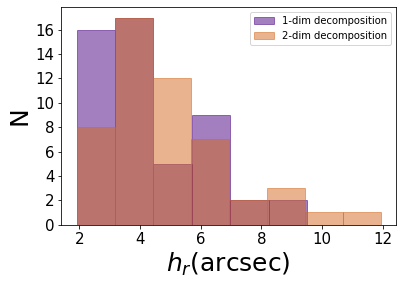
\includegraphics[width=.5\textwidth]{plot_results/h_arcsec.png}\hfill
    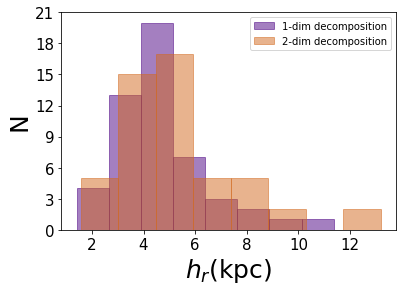
\includegraphics[width=.5\textwidth]{plot_results/h_kpc.png}\hfill\\
    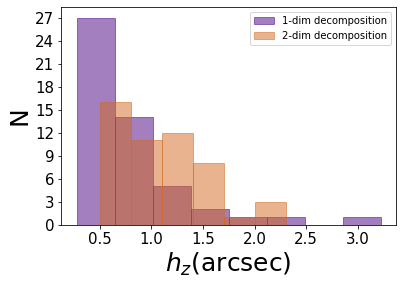
\includegraphics[width=.5\textwidth]{plot_results/h_z_arcsec.png}\hfill
    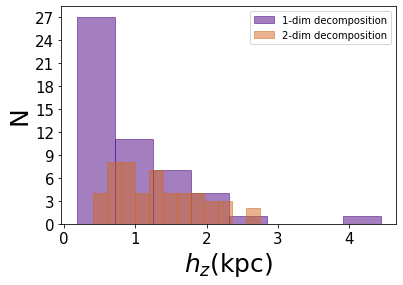
\includegraphics[width=.5\textwidth]{plot_results/h_z_kpc.png}\hfill\\

    \caption{Распределения по радиальным и вертикальным масштабам дисков галактик, выраженные в угловых секундах (левая панель) и в килопарсеках (правая панель). Цвет обозначает тип декомпозиции, в результате которой получены данные параметры: фиолетовый -- одномерная декомпозиция, оранжевый -- двумерная декомпозиция.}\label{fig:hz_hist}
\end{figure}

Получены средние значения радиальных масштабов диска: $\langle h \rangle_{1d}$ = $4.29 \pm 0.25$ arcsec и $\langle h \rangle_{2d}$ = $4.89 \pm 0.28$ arcsec, для одномерной и двумерной декомпозиции (в качестве ошибки здесь и далее приведено значение выборочной дисперсии).
Средние значения вертикальных масштабов диска $\langle h_z \rangle$ равны $0.79 \pm 0.08$ arcsec и $1.13 \pm 0.05$ arcsec также для одномерной и двумерной декомпозиции соответственно. Аналогично посчитаны
средние значения радиальных и вертикальных масштабов диска, выраженные в килопарсеках: $\langle h \rangle_{1d}$ = $4.72 \pm 0.27$ kpc и $\langle h \rangle_{2d}$ = $5.41 \pm 0.32$ kpc, для одномерной и двумерной декомпозиции. 
Средние значения вертикальных масштабов диска $\langle h_z \rangle$ равны $0.46 \pm 0.05$ kpc и $0.65 \pm 0.04$ kpc  для одномерной и двумерной декомпозиции соответственно. 
Приведенные значения масштабов выглядят типичными для наблюдаемых в ориентации с ребра близких галактик (см., например,
рис. 10 в \cite{2014ApJ...787...24B}).

Для получения значений масштабных параметров в килопарсеках из базы данных SDSS были взяты значения спектральных красных смещений для галактик выборки. При помощи красных смещений, используя пакет IMAN, мы смогли определить значения масштабов, связывающих размеры объектов, выраженные в угловых секундах с размерами, выраженными в килопарсеках. Распределение по красным смещениям для нашей выборки представлено на рис. \ref{fig:z_spec}. Все числовые величины в работе приведены для космологической
модели с постоянной Хаббла $H_0=70км\,c^{-1}\,\textrm{Мпк}^{-1}$, $\Omega_m=0.3, \Omega_{\Lambda}=0.7$.
\begin{figure}[th]
    \centering
    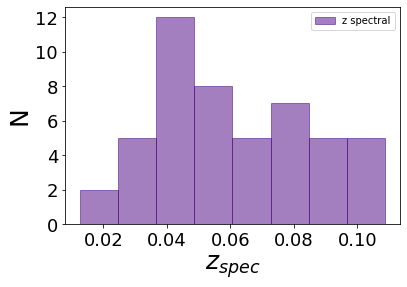
\includegraphics[width=.8\textwidth]{plot_results/z_spec.png}
    \caption{Распределение по спектральным красным смещениям галактик выборки, полученные из базы данных SDSS в фильтре r. }\label{fig:z_spec}
\end{figure}
Среднее красное смещение рассматриваемых нами галактик составляет $\langle z_{spec} \rangle$ = $0.064 \pm 0.004$. Галактики являются достаточно далекими для того, чтобы при дальнейших расчетах абсолютных звездных величин помимо галактического поглощения также учитывать значение К-поправки.

Распределение галактик по абсолютным звездным величинам (M) приведены на рис. \ref{fig:M_abs}.
\begin{figure}[th]
    \centering
    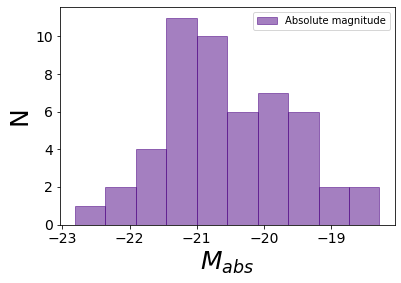
\includegraphics[width=.9\textwidth]{plot_results/M_abs.png}
    \caption{Распределение по абсолютным звездным величинам в фильтре r, расчитанным для модельных галактик. }\label{fig:M_abs}
\end{figure}
Абсолютные звездные величины были вычислены по формуле \ref{eq:M_abs}:
\begin{equation}
    M = m_{model}-5\log(D_L^{Mpc})-25-A-K,
    \label{eq:M_abs}
\end{equation}
Где $\textrm{ }m_{model}$ -- видимая звездная величина модельной галактики, $D_L^{Mpc}$(lumonocity distance) $=\sqrt{{\frac{L}{4\pi F}}}$ (где L -- светимость, F -- поток). Для расчета K-поправок использовался скрипт I. Chilingarian, A.-L. Melchior, and I. Zolotukhin. \footnote{http://kcor.sai.msu.ru/getthecode/}
Среднее значение M для галактик выборки: $\langle M \rangle_{2d}$ = $-20.53 \pm 0.13$, что согласуется с результатами работы \citep{2014ApJ...787...24B}.

% Изучаемая нами выборка видимых с ребра галактик в полосе Stripe 82 неполна. Эта неполнота должна сильнее всего проявляться для слабых и плохо разрешаемых галактик, у которых сложно определить ориентацию звездных дисков по отношению к лучу зрения.
О том, насколько галактика имеет тонкий звездный диск мы также можем судить по наблюдениям галактик, видимых с ребра. В большинстве своем, данная характеристика представляет собой отношения двух масштабных параметров \textit{h} и $z_0$ или \textit{h} и $h_z$. Существует четкая корелляция между этими двумя параметрами, что подтверждалось, например, в работах \citep{2002MNRAS.334..646K} или \citep{2010MNRAS.401..559M}. В нашей работе эта корреляция также присутствует (см. рис.\ref{fig:hr_z_0}). Примечательно, что продолжение линейной регрессии проходит вблизи точки с координатами (0, 0). 

Мы также построили распределение толщин звездных дисков для одномерной и двумерной декомпозиции \ref{fig:hr_hz_hist}. Видим, что существует большой разброс значений $h/z_0$ по результатам одномерной декомпозиции, в то время, как $h/z_0$ для двумерной декомпозиции ограничивается значением$\approx$ 9.5. Считаем, что данная несостыковка произошла из-за неточного определения значения $z_0$ в процессе одномерной декомпозиции, как минимум значения толщин $h/z_0 \approx$ 20.0 -- нефизичны. Еще одно подтверждение того, что одномерную декомпозицию лучше использовать исключительно в качестве начального приближения для двумерной.  
\begin{figure}[th]
    \centering
    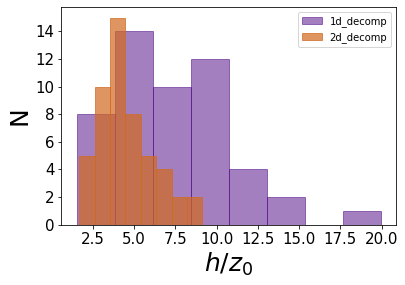
\includegraphics[width=.8\textwidth]{plot_results/h_z0_hist.png}
    \caption{Распределение галактик по значениям толщин звездных дисков. Фиолетовая гистограма демонстрирует параметры, полученные в процессе одномерной декомпозиции, оранжевая гистограмма -- в процессе двумерной. }\label{fig:hr_hz_hist}
\end{figure}

\begin{figure}[th]
    \centering
    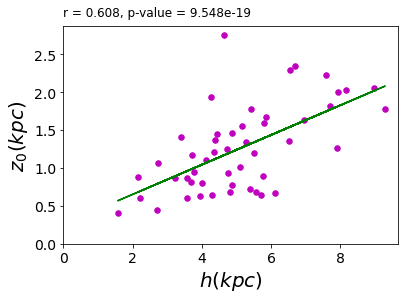
\includegraphics[width=.8\textwidth]{plot_results/h_r_z_0.png}
    \caption{Распределение галактик на плоскости $h$ $h_z$, зеленая сплошная линия -- линейная регрессия для данной выборки галактик, r -- коэффициент Пирсона, p -- p-значение. }\label{fig:hr_z_0}
\end{figure}

Заключительный и наиболее важный раздел анализа, выполненный в рамках данной работы, это анализ толщин звездных дисков галактик в зависимости от наличия или отсутствия у тех приливных структур. Из теоретических соображений следует, что толщина звездных дисков чувствительна к внешнему возмущению и аккреции вещества \cite{1992ApJ...389....5T}. При гравитационном взаимодействии галактик, в частности, при малых и больших слияниях, часть энергии орбитального движения галактик может преобразоваться в их внутреннюю энергию, "разогреть"$\textrm{ }$ звездные диски, тем самым увеличив дисперсию скоростей звезд в вертикальном направлении, следовательно, и наблюдаемую толщину. Эффект приливного утолщения был, действительно, открыт при сравнении распределений яркости в вертикальном направлении в выборках взаимодействующих и относительно изолированных галактик в работе \citep{1997A&A...324...80R}. Было продемонстрировано, что галактики во взаимодействующих системах демонстрируют в 1.5-2 раза более толстые диски по сравнению с галактиками в более бедном пространственном окружении. Мы решили проверить этот факт на нашей выборке. В данном случае речь идет о всем каталоге галактик EG82, содержащем 831 объект, так мы имеем возможность учесть все галактики из предыдущего раздела, посвященного приливным структурам. В качестве критерия оценки толщин дисков мы будем использовать отношение полуосей \textit{b/a}. Соответственно, чем меньше это соотношение, тем тоньше диск, и на оборот. На 831 объект выборки у нас приходится 43 галактики с наблюдаемыми приливными структурами. Мы построили распределение толщин для двух подвыборок: галактик с приливными структурами и оставшейся части выборки (788 объектов) (см. рис. \ref{fig:b_a}.) 
\begin{figure}[th]
    \centering
    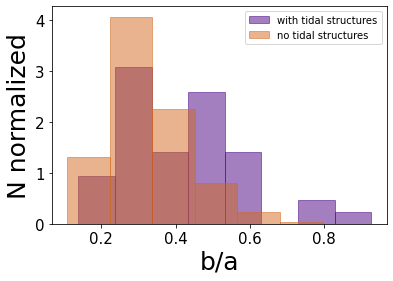
\includegraphics[width=.8\textwidth]{plot_results/b_a.png}
    \caption{Распределение толщин галактик (отношение малой полуоси к большой) для двух выборок галактик: фиолетовая гистограмма для галактик с наблюдаемыми приливными структурами, оранжевая гистограмма для галактик с отсутствующими приливными структурами.}\label{fig:b_a} 
\end{figure}

Среднее значение толщины диска для выборки с приливными структурами -- $\langle b/a \rangle_{2d}$ = $0.412 \pm 0.03$, в то время, как для выборки галактик, у которых приливные структуры отсутствуют это же значение равно  $\langle b/a \rangle_{2d}$ = $0.325 \pm 0.003$. Не в два раза, но все равно диски галактик со структурами заметно толще дисков визуально не взаимодействующих галактик.
    % \item Исходя из графика, представленного на рисунке (??) мы можем сделать вывод о наличие корелляции между параметрами $h_r$ и $z_0$. Отметим тот факт,что график линейной функции, аппроксимирующий распределение в пространстве данных параметров проходит через точку, близкую к точке с координатами (0,0).  Среднее значение отношения $h_r/z_0$ для одномерной и двумерной декомпозиции: $\langle h_r/z_0 \rangle_{1d}=$  $7.40 \pm 0.43$ и $\langle h_r/z_0 \rangle_{1d} =$  $4.97 \pm 0.23$.
    % \item 
